\section{Demand Forecasting Model}

\subsection{Forecasting Approach}

In this work, the Prophet forecasting model is utilized to forecast the future demand in the sales of the third-party delivery platform. Prophet is chosen as it is suitable with business time series data and can process typical patterns like trends and seasonality. 

The possibility to model the time series data having a high seasonal influence, e.g. daily and weekly trends is one of the primary reasons why Prophet is selected. This feature can be especially helpful in the case of food delivery platforms, where demand tends to change on a weekly basis. Prophet is able to automatically record these patterns without the need to make any manual adjustments. 

The other strength of Prophet is that it can withstand missing data and outliers. Sales data in real-life scenarios tend to have anomalies and Prophet is set to manage these anomalies. This renders it viable to use in business applications in which data might not be exactly clean. 

Also, Prophet can be implemented and interpreted easily as opposed to other more complicated machine learning models. It has well-defined elements like trend and seasonality that can be used to explain how the model has come up with forecasts. The transparency is necessary in terms of decision-making and reporting the outcomes to the stakeholders. 

Lastly, Prophet works reasonably well with rather small data and involves little parameter optimization. This renders it appropriate in this study, in which the objective is to come up with a robust and useful forecasting model to be used in decision-support. In general, Prophet is selected as it is accurate, simple, and interpretable and is a suitable tool in forecasting the platform-level demand in this study.


\subsection{Model Specification}

The Prophet model decomposes the time series into several key components, mainly trend, seasonality, and holiday effects. These components help capture different patterns in the data and improve forecasting accuracy.

\textbf{Trend Component}

The trend component is the long term trend of the time series. It shows
whether the level of orders is tending upwards, downwards, or is in a steady state over time. Prophet fits a piecewise linear or logistic growth function to model the trend to enable it to record both incremental and abrupt changes in the data. This is important of business data in which demand can vary based on market conditions or business.
strategies.

\textbf{Seasonality}

Seasonality reflects recurring patterns, which are periodically repeated. Weekly seasonality is especially significant in this research because the behavior of customers in terms of ordering can be very different on different days of the week. As an illustration, the demand can be greater during the weekends than weekdays. Prophet uses flexible functions to automatically model these seasonal patterns thus enabling it to capture and model changes in demand which are periodic.

\textbf{Holiday Effects}

Holiday effects explain unusual events that might have an impact on the demand like a special occasion or a public holiday. The behavior of customers during such times can be far off the normal trend and as a result, orders may peak or decline. Prophet enables consideration of the variables of holidays to modify the forecasts. Holiday effects may be used in this study provided that there is the relevant data, but its effect may be minimal depending on the data.


\subsection{Forecast Results}

This section presents the results obtained from the Prophet forecasting model. The results are analyzed through trend, seasonality, and forecasted demand to understand future sales behavior.

\textbf{Trend Analysis}

The trend component shows the overall direction of demand over time. Based on the Prophet model, the trend indicates a slight downward pattern in the number of orders over the observed period. This suggests that, on average, demand is gradually decreasing, although short-term fluctuations still occur.

Figure~\ref{fig:trend_component} illustrates the estimated trend component from the model.

\begin{figure}[h]
\centering
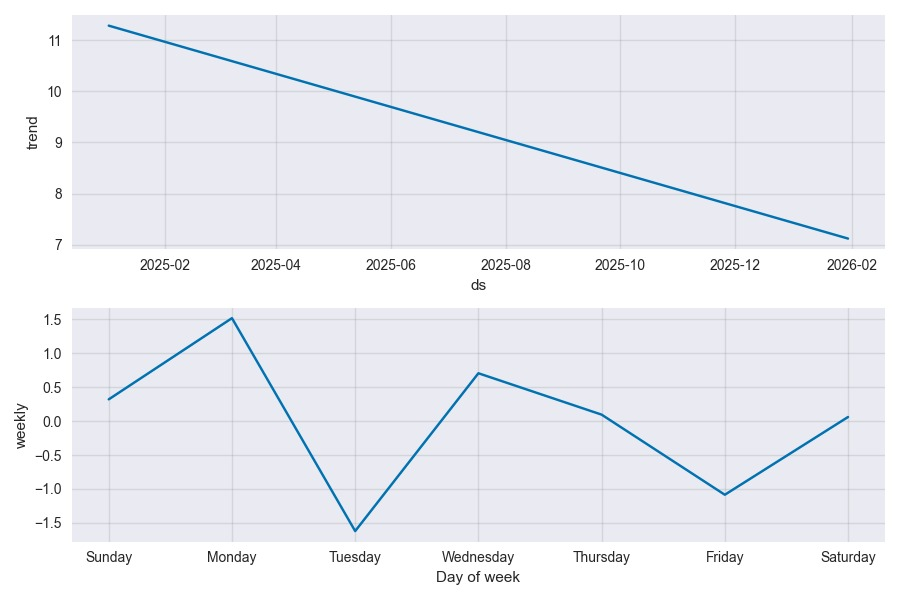
\includegraphics[width=0.8\textwidth]{figures/2.jpeg}
\caption{Trend Component from Prophet Model}
\label{fig:trend_component}
\end{figure}


\textbf{Weekly Seasonality}

The weekly seasonality component captures how demand changes across different days of the week. The results show that demand is higher on certain days (such as weekends or early weekdays) and lower on others. For example, Monday and Wednesday may show higher demand, while Tuesday and Friday show lower demand.

This pattern reflects customer behavior and is important for understanding recurring demand cycles.

Figure~\ref{fig:weekly_seasonality} presents the weekly seasonal pattern.

\begin{figure}[h]
\centering
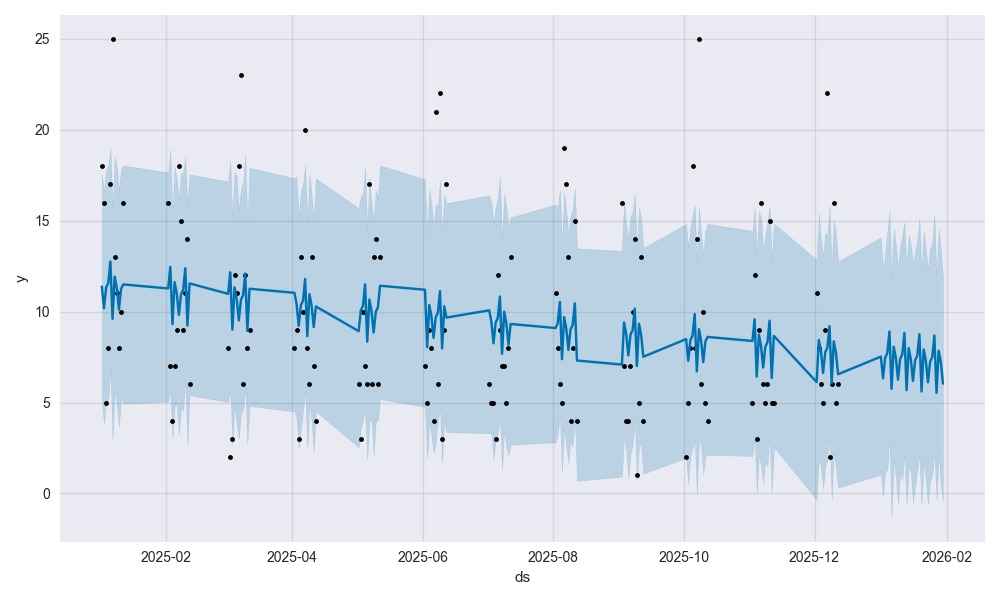
\includegraphics[width=0.9\textwidth]{figures/3.jpeg}
\caption{Weekly Seasonality from Prophet Model}
\label{fig:weekly_seasonality}
\end{figure}


\textbf{Forecasted Demand}

The forecasted demand shows the predicted number of orders for the future period. The model predicts relatively stable demand with moderate fluctuations, typically ranging within a consistent interval. Compared to historical data, the forecast appears smoother, indicating that the model reduces random noise while capturing underlying patterns.

Figure~\ref{fig:forecast} shows the full forecast, including historical data, predicted values, and confidence intervals.

\begin{figure}[h]
\centering
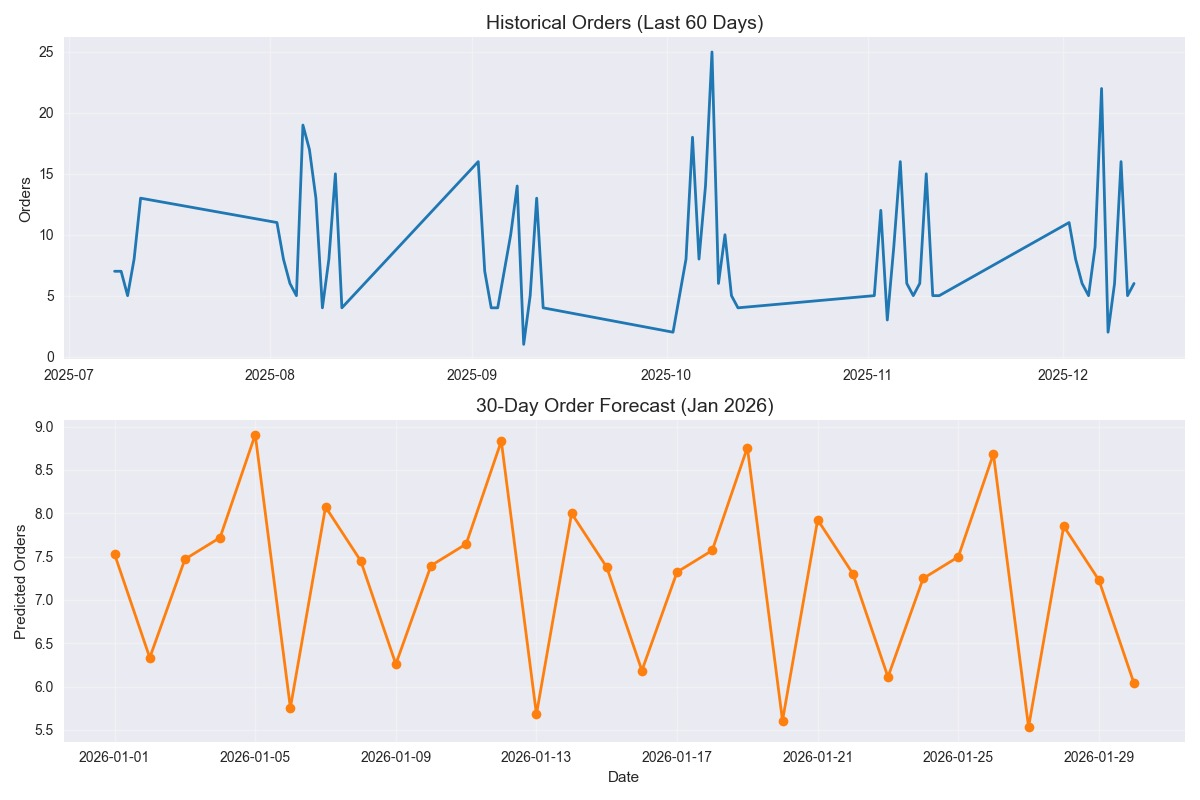
\includegraphics[width=1.0\textwidth]{figures/4.jpeg}
\caption{Forecasted Demand using Prophet}
\label{fig:forecast}
\end{figure}

Overall, the results demonstrate that the Prophet model effectively captures trend and seasonal patterns while providing reliable forecasts for future demand.


\subsection{Forecast Accuracy Evaluation}

To evaluate the performance of the forecasting model, several standard accuracy metrics are used. These metrics compare the predicted values with the actual observed values and help assess how well the model performs.

\begin{table}[h]
\centering
\begin{tabular}{|p{4cm}|p{4cm}|p{6cm}|}
\hline
\textbf{Metric} & \textbf{Definition} & \textbf{Description} \\
\hline
MAE (Mean Absolute Error) & Average of absolute differences between actual and predicted values & Measures overall prediction error in simple terms. Easy to interpret. Lower values indicate better accuracy. \\
\hline
RMSE (Root Mean Squared Error) & Square root of average squared differences between actual and predicted values & Penalizes larger errors more than MAE. Sensitive to outliers. Lower values indicate better performance. \\
\hline
MAPE (Mean Absolute Percentage Error) & Average percentage difference between actual and predicted values & Expresses error as a percentage, making it easy to understand and compare. Can be sensitive when actual values are very small. \\
\hline
\end{tabular}
\caption{Forecast Accuracy Metrics}
\end{table}